\subsection{Parallel Vs. Serial Performance}
After having implmented the MPI methods into the serial solver the performance was plotted in \fig\ref{fig:large:MPIVTOTAL} below. 
\definecolor{mycolor1}{rgb}{0.750, 0.750, 0.750} % lighter shade 
\begin{figure}[H]
    \begin{minipage}[t]{0.45\linewidth}
        \centering
        \includegraphics[height=6.5cm,width=\linewidth]{Images/\largedomain___MPIVTOTAL.png}
        \caption{Plot showing performance of MPI implementation against serial case}
        \label{fig:large:MPIVTOTAL}
    \end{minipage}
    \hspace{0.5cm}
    \begin{minipage}[t]{0.45\linewidth}
        \vspace*{-2cm}
        \begin{table}[H]
            \centering
            \small
            \caption{Settings used when investigating parallel vs. serial performance}
            \begin{tabular}{@{}llllllll@{}}
            \hline
            \textit{\textbf{Profile}} & \textit{\textbf{Lx}} & \textit{\textbf{Ly}} & \textit{\textbf{Nx}} & \textit{\textbf{Ny}} & \textit{\textbf{Re}} & \textit{\textbf{dt}} & \textit{\textbf{T}} \\ \hline
            % Fine dt                   & 1.00                 & 1.00                 & 201                  & 201                  & 10                  & \cellcolor{mycolor1}0.00005                & 0.00500               \\
            % Coarse dx dy              & \cellcolor{mycolor1}10.00                & \cellcolor{mycolor1}10.00                & 201                  & 201                  & 1000                 & 0.005                & 5.000               \\
            Large                     & 1.00                 & 1.00                 & \cellcolor{mycolor1}201                  & \cellcolor{mycolor1}201                  & 1000                  & 0.005                & 5.000               \\
            % Medium                 & 1.00                 & 1.00                 & \cellcolor{mycolor1}151                  & \cellcolor{mycolor1}151                  & 1000                  & 0.001                & 1.000               \\
            Small                     & 1.00                 & 1.00                 & \cellcolor{mycolor1}101                  & \cellcolor{mycolor1}101                  & 500                  & 0.005                & 5.000                                  
            \end{tabular}
            \label{tab:settings}
        \end{table}
    \end{minipage}
\end{figure}

% \begin{figure}[H]
%         \centering
%         \includegraphics[height=6.5cm,width=0.45\textwidth]{Images/\largedomain___MPIVTOTAL.png}
%         \caption{Plot showing performance of MPI implementation against serial case}
%         \label{fig:large:MPIVTOTAL}
% \end{figure}
\vspace{-0.75cm}
The scaling plot above was produced with the ``Large'' settings found above in \tabl\ref{tab:settings}. These paramters were chosen to ensure a large enough domain to take advantage of the number of ranks available.
The main setting change of note for a given profile was highlighted above.
% \begin{table}[H]
%     \centering
%     \caption{Settings used when investigating parallel vs. serial performance}
%     \label{tab:settings}
%     \begin{tabular}{@{}llllllll@{}}
%         \toprule
%         \multicolumn{1}{c}{\textit{\textbf{Profile}}} & \multicolumn{1}{c}{\textit{\textbf{Lx}}} & \multicolumn{1}{c}{\textit{\textbf{Ly}}} & \multicolumn{1}{c}{\textit{\textbf{Nx}}} & \multicolumn{1}{c}{\textit{\textbf{Ny}}} & \multicolumn{1}{c}{\textit{\textbf{Re}}} & \multicolumn{1}{c}{\textit{\textbf{dt}}} & \multicolumn{1}{c}{\textit{\textbf{T}}} \\ \midrule
%         % Fine dt                   & 1.00                 & 1.00                 & 201                  & 201                  & 10                  & \cellcolor{mycolor1}0.00005                & 0.00500               \\
%         % Coarse dx dy              & \cellcolor{mycolor1}10.00                & \cellcolor{mycolor1}10.00                & 201                  & 201                  & 1000                 & 0.005                & 5.000               \\
%         Large                     & 1.00                 & 1.00                 & \cellcolor{mycolor1}201                  & \cellcolor{mycolor1}201                  & 1000                  & 0.005                & 5.000               \\
%         % Medium                 & 1.00                 & 1.00                 & \cellcolor{mycolor1}151                  & \cellcolor{mycolor1}151                  & 1000                  & 0.001                & 1.000               \\
%         Small                     & 1.00                 & 1.00                 & \cellcolor{mycolor1}101                  & \cellcolor{mycolor1}101                  & 500                  & 0.005                & 5.000                                  
%     \end{tabular}
% \end{table}

Through testing at other settings, similar plots were made (found in \app\ref{Appendix::Support}), and it was seen that the smaller the spatial domain the worse the scaling appeared.
This was due to the increase in relative communication time between neighbour ranks. When a smaller grid was chosen, more time was spent communicating between ranks relative to actually doing computation on their local vectors.
Furthermore, from the figure it can be seen that the increase in ranks from serial case does flatten off in terms of reduction in total time. This will be due to both the domain size, not utilising the maximum number of ranks (16) as efficiently as possible;
and primarily, that the communication overhead through the increase in calls to exchange information between neighbour ranks (seen in \code\ref{lst:PFCpp}) became detrimental to performance.  

To compare the relative reductions in timings of the main components of the main program, a normalised time reduction scaling plot was produced, as seen below in \fig\ref{fig:both:MPIVNORMAL}.
\vspace{-0.5cm}
\begin{figure}[H]
    \centering
    \begin{subfigure}[b]{0.45\textwidth}
        \centering
        \includegraphics[height=6.5cm,width=\textwidth]{Images/\largedomain___MPIVNORMAL.png}
        \caption{MPI (Large)}
        \label{fig:large:MPIVNORMAL}
    \end{subfigure}
    \hfill
    \begin{subfigure}[b]{0.45\textwidth}
        \centering
        \includegraphics[height=6.5cm,width=\textwidth]{Images/\smalldomain___MPIVNORMAL.png}
        \caption{MPI (Small)}
        \label{fig:small:MPIVNORMAL}
    \end{subfigure}
    \caption{Plots showing normalized time scaling plot to see the effect MPI parallelisation has on both ``Large'' and ``Small'' domains}
    \label{fig:both:MPIVNORMAL}
\end{figure}
\vspace{-0.5cm}
As mentioned earlier its clear that the reduction in solve time was greater with the larger domain. From \fig\ref{fig:large:MPIVNORMAL} we see a 82\% reduction in ``Solve'' time with 9 ranks compared to the serial case. However, for the ``Small'' paramters, \fig\ref{fig:small:MPIVNORMAL} respectively shows 64 \% reduction.
Furthermore, this plot also shows a similar level of gains in the across both settings with the ``Initialise'' function which was used when allocating the local vectors with dynamic memory and creating the ``dataGrid'' objects.
Shown in both figures, it is clear that the writing to ``.txt'' file operations maintained a constant time within increasing rank number, accounting for variance.
This was due to the fact that when converting this operation from serial to parallel, it was deemed efficient to instead synchronously iterate over the global grid and only print the associated data from the correct rank.
This approach was taken in order to avoid regathering all data, rendering the distribution of work / memory pointless.  

\subsection{Design Methodology}
The source code for the grid implemntation can be found in the ``prl::dataGrid'' struct in \app\ref{Appendix::Parallel}.
The extending of the serial code to utilise a square number of MPI ranks, primarily focused on the implemntation of a virtual topology.
As seen in \fig\ref{fig:CartGrid}, the global grid defined by the $L_x,L_y,N_x\textnormal{ and }N_y$ parameters had to be divided as evenly as possible to ensure the load was balanced and the computations were distributed as evenly as possible amongst the ranks.
Using the logic found in the method ``gridData::init'', the grid was divided into chunks along both dimensions.
\begin{figure}[H]
    \centering
    \begin{subfigure}[b]{0.3\textwidth}
        \centering
        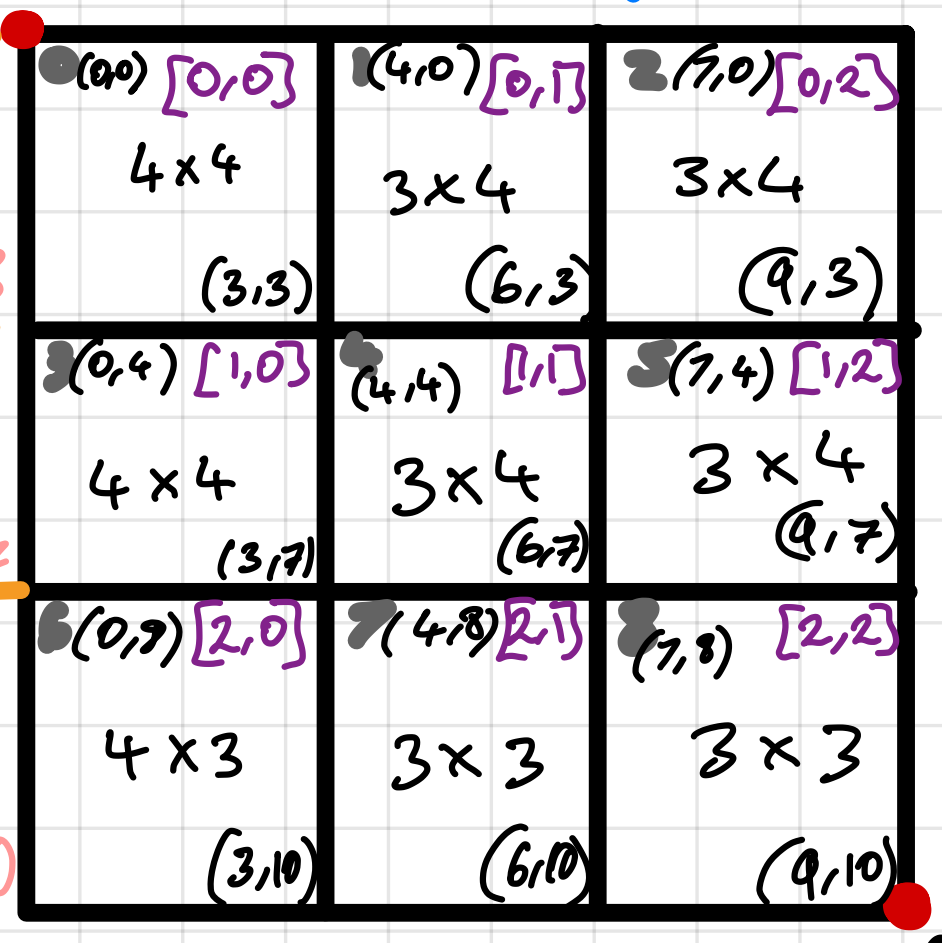
\includegraphics[height=4.5cm,width=\linewidth]{Images/CartGrid.png}
        \caption{Initial concept for grid with each MPI rank having local and global coordinates}
        \label{fig:CartGrid}
    \end{subfigure}
    \hfill
    \begin{subfigure}[b]{0.3\textwidth}
        \centering
        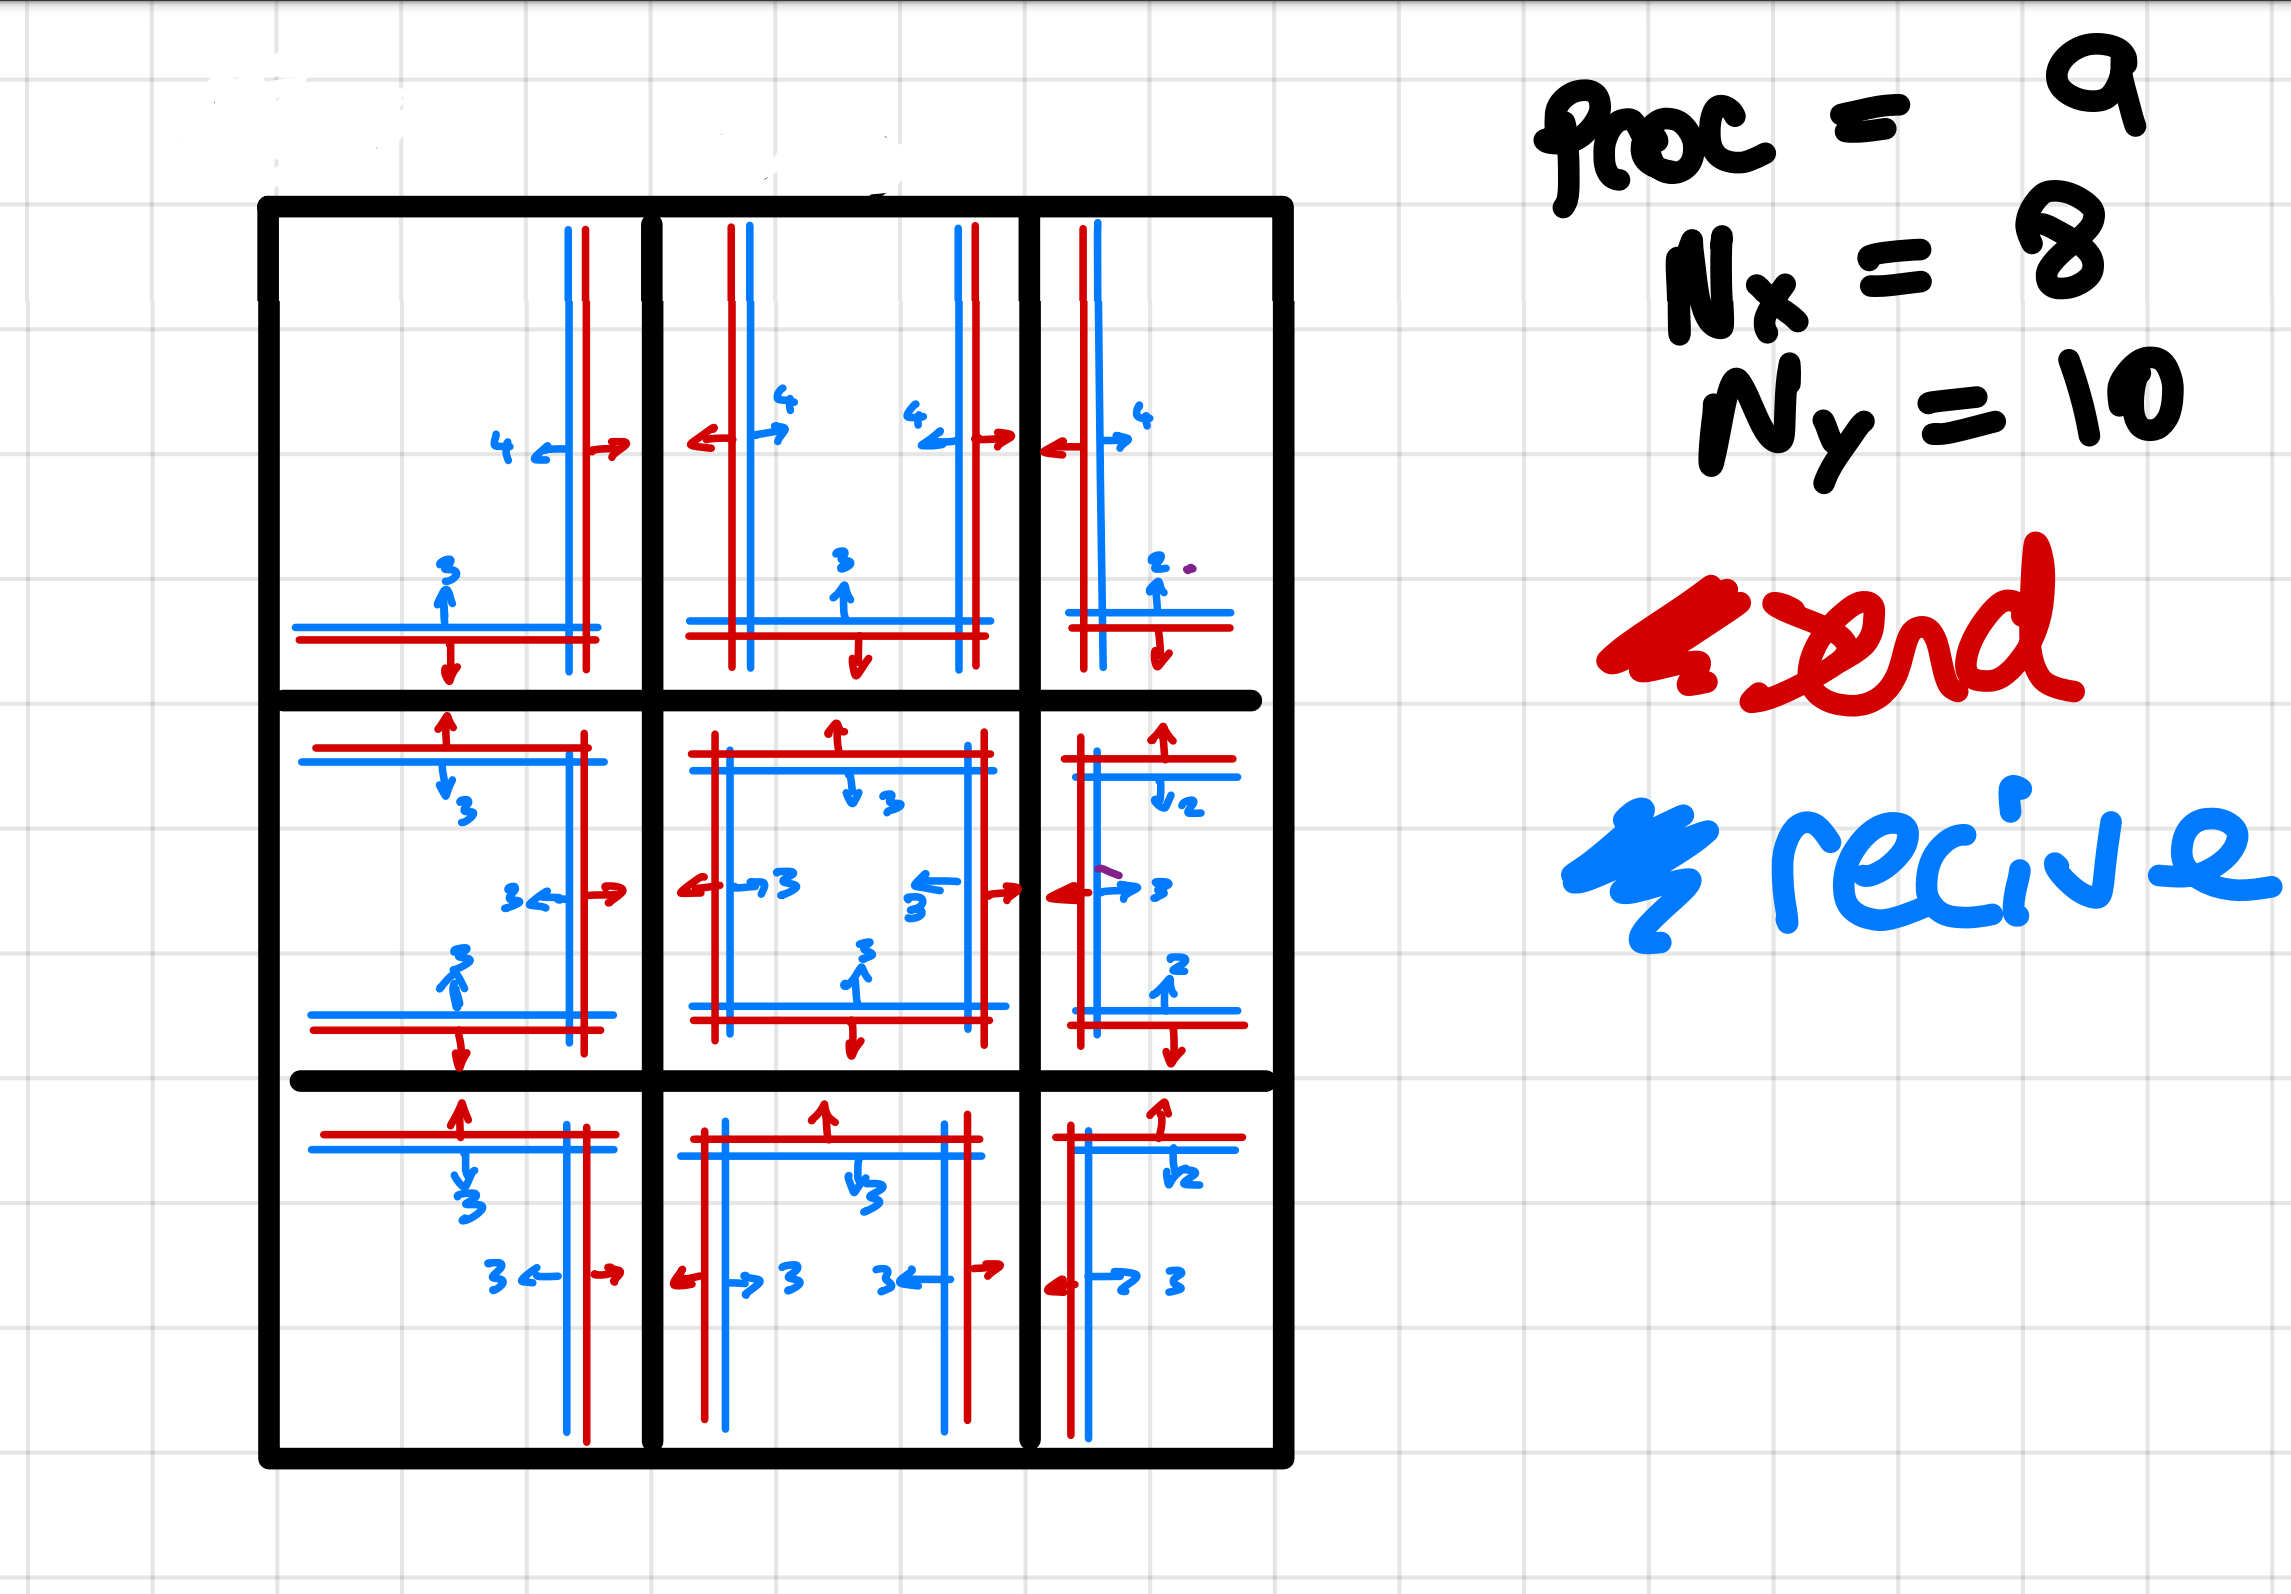
\includegraphics[height=4.5cm,width=\linewidth]{Images/ExchangeDiagram.png}
        \caption{Diagram detailing information exchange between MPI ranks}
        \label{fig:ExchangeDiagram}
    \end{subfigure}
    \hfill
    \begin{subfigure}[b]{0.3\textwidth}
        \centering
        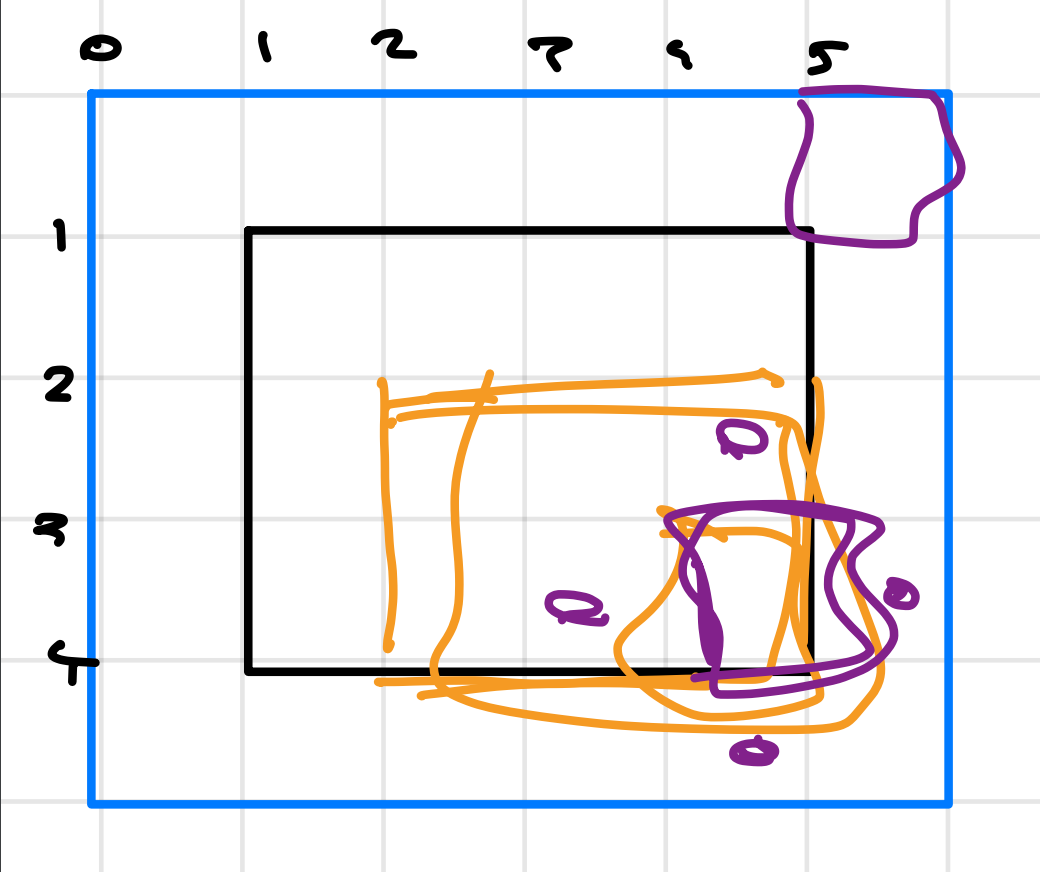
\includegraphics[height=4.5cm,width=\linewidth]{Images/Padding.png}
        \caption{Diagram of local vectors with padding in each MPI rank for vorticity and stream function}
        \label{fig:Padding}
    \end{subfigure}
    \caption{Diagrams detailing MPI development conceptual process and implementation}
    \label{fig:Parallel}
\end{figure}
\vspace{-0.5cm}
Moreover, when initialising the grid, each rank with the use of the ``gridData'' object could store information such as its global coordiantes for its top-left and bottom-right corners and its neighbour ranks.
This data was extremely useful when the exchange of edge values became necessary between neighbour ranks, which can be seen in \code\ref{lst:PFCpp}. 
As seen in \fig\ref{fig:ExchangeDiagram}, each rank had to know to only send to an available neighbour and send and data with the same size dimensions.
This was implemented using non-blocking send and receive messages (``MPI\_Isend'' and ``MPI\_Irecv'') to ensure there was no wasted time between sending to the neighbour above and to the right, as the information didnt depend on each other.
Shown in \fig\ref{fig:Padding}, each local vector was actually stored with padding to allow receives of neighbour data, and to keep numerical scheme funcions consistent.
However, to ensure that the current rank had the information necessary to move on in the program, a ``MPI\_WAITALL'' was implemented utilising ``MPI\_REQUEST'' objects.
Furthermore, to ensure all resources created by MPI were deallocated, ``MPI\_REQUEST\_FREE'' calls were implemented for the send requests, whilst the wait function freed the receive requests automatically.
\subsubsection{LidDrivenCavity}
The main efforts to parallelise the code in the LDC class, was to work on the ``Advance'' method. Here when operating on the vorticity vector, the parallel code could perfrom well.
Through the use of checks whether the current rank had no neighbour in a direction implied whether the rank was at a wall. Therefore, when computing different schemes based of that information,
the rank only operated on the correct data. For example, when considering the ``interior'' points schemes with calculating and advancing vorticity, the rank had to check if they were at walls and such only operate on their own local ``interior'' data.
This was acheived through a ternary operator in the inital and final loop counter values, shown in \code\ref{lst:LDC}.
\subsubsection{SolverCG}
On the other hand, within the SCG class, there were much more opportunities to take advantage of the distribution of work.
Significantly, all the function calls using BLAS were improved due to their reduced vector size. Furthermore, the operations involving imposing boundary conditions, and applying the matrix operation of $Ax$ were significantly imrpoved as the size of the for loops reduced as the number of ranks increased.
One thing to note was that the calculations using parameters like $\alpha$ and $\beta$ had to be locally computed and reduced to all ranks before being used, to maintain the same serial logic  as before.
